\ExamPart{Trắc nghiệm trả lời ngắn}{2}{Thí sinh trả lời từ câu 1 đến câu 4.}

\NQuestion Cho đồ thị hàm số $y=f(x)$ như hình vẽ dưới đây.
\begin{center}
    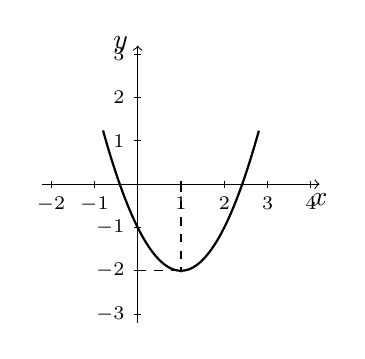
\begin{tikzpicture}[scale=0.55]
    \draw[->] (-2.2,0) -- (4.2,0) node[below] {$x$};
    \draw[->] (0,-3.2) -- (0,3.2) node[left] {$y$};
    \foreach \x in {-2,-1,1,2,3,4}
      \draw (\x,0.08)--(\x,-0.08) node[below] {\scriptsize $\x$};
    \foreach \y in {-3,-2,-1,1,2,3}
      \draw (0.08,\y)--(-0.08,\y) node[left] {\scriptsize $\y$};
    \draw[smooth, samples=200, domain=-0.8:2.8, thick] plot (\x, {(\x-1)^2-2});
    \fill (1,-2) circle (1.2pt);
    \draw[dashed] (1,0)--(1,-2);
    \draw[dashed] (0,-2)--(1,-2);
\end{tikzpicture}

\end{center}
Tìm giá trị nhỏ nhất của hàm số.
\AnswerLine{$-2$}
\SolutionBlock{Từ đồ thị, parabol mở lên và có đỉnh là $I(1;-2)$, nên giá trị nhỏ nhất là $-2$.}

\NQuestion Phương trình $x^4-13x^2+36=0$ có bao nhiêu nghiệm thực phân biệt?
\AnswerLine{$4$}
\SolutionBlock{Đặt $t=x^2\ (t\ge0)$, ta được
\[
t^2-13t+36=0\Leftrightarrow (t-4)(t-9)=0.
\]
Suy ra $t=4$ hoặc $t=9$, nên $x=\pm2,\pm3$. Vậy có $4$ nghiệm thực phân biệt.}

\NQuestion Một đoàn du lịch có $8$ điểm tham quan. Trong một ngày, đoàn chỉ chọn tham quan đúng $3$ điểm và thứ tự đi các điểm có ý nghĩa. Hỏi có bao nhiêu lịch trình có thể chọn?
\AnswerLine{$336$}
\SolutionBlock{Vì thứ tự đi có ý nghĩa nên đây là chỉnh hợp chập $3$ của $8$ phần tử:
\[
A_8^3=8\cdot7\cdot6=336.
\]}

\NQuestion Một sân bóng hình chữ nhật có chiều dài hơn chiều rộng $7$ m và diện tích bằng $144$ m$^2$. Tính chu vi sân bóng.
\AnswerLine{$50$}
\SolutionBlock{Gọi chiều rộng là $x$ m, chiều dài là $x+7$ m. Khi đó
\[
x(x+7)=144\Rightarrow x^2+7x-144=0\Rightarrow (x+16)(x-9)=0.
\]
Suy ra $x=9$ (nhận), chiều dài là $16$. Chu vi là
\[
2(9+16)=50.
\]}
